An angle is drawn on a set of equally spaced parallel lines as shown.  The ratio of the area of shaded region $\mathcal{C}$ to the area of shaded region $\mathcal{B}$ is $11/5$.  Find the ratio of shaded region $\mathcal{D}$ to the area of shaded region $\mathcal{A}$.

\begin{center}
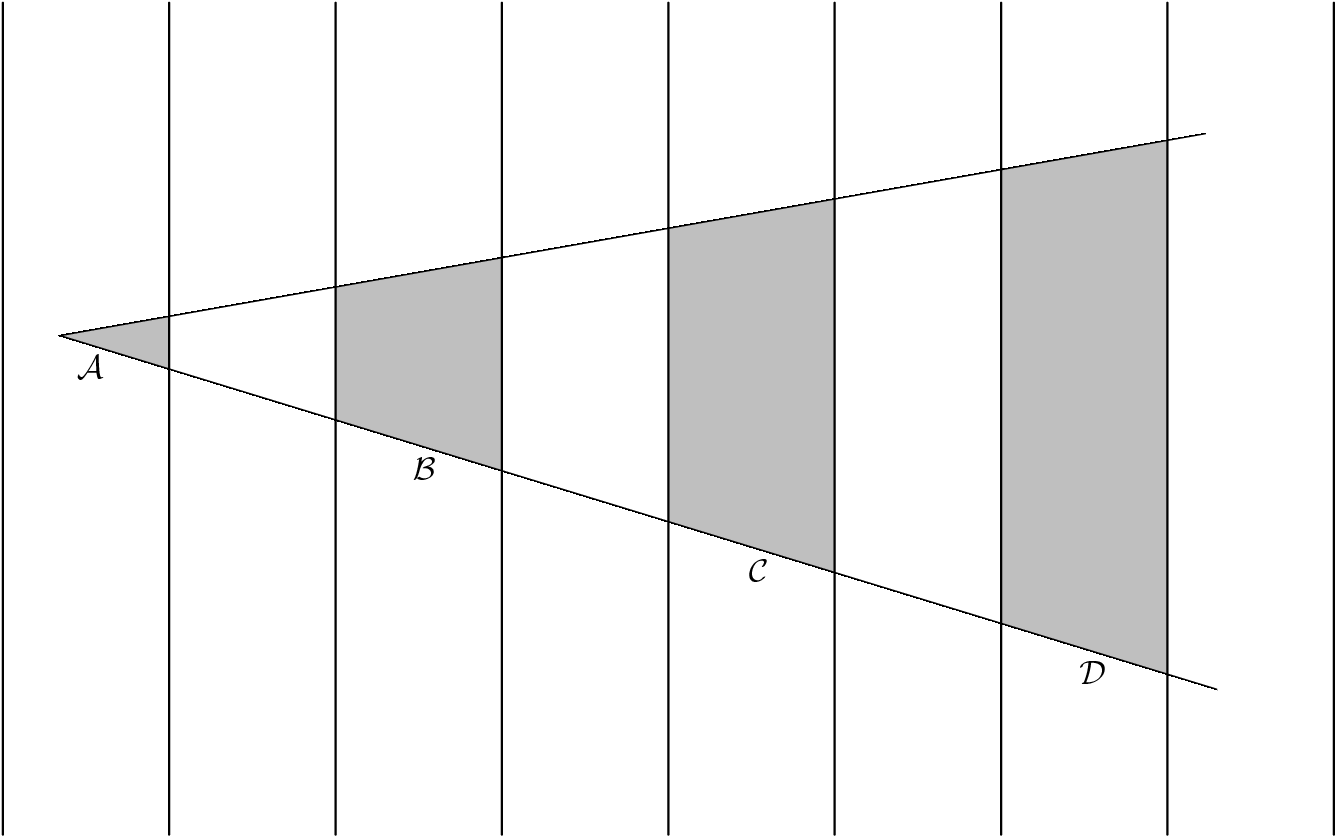
\includegraphics[width = 133.6mm]{img/fig0.png}
\end{center}